% Preamble
\documentclass[10pt,reqno,oneside,a4paper]{article}
\usepackage[a4paper,includeheadfoot,left=25mm,right=25mm,top=00mm,bottom=20mm,headheight=20mm]{geometry}
\usepackage[toc,page]{appendix}
\usepackage{siunitx}
\usepackage{caption}
\usepackage{subcaption}
% Standard packages
\usepackage{amssymb,amsmath,amsthm}
\usepackage{xcolor,graphicx}
\usepackage{verbatim}
\usepackage{hyperref}
% To use turkish characters
\usepackage[utf8]{inputenc}
% Layout of headers & footers
\usepackage{titling}
\usepackage{fancyhdr}
\pagestyle{fancy} \lhead{{\theauthor}} \chead{} \rhead{{\theshorttitle}} \lfoot{} \cfoot{\thepage} \rfoot{}

% Hyphenation
\hyphenation{non-zero}

% Theorem definitions in the amsthm standard
\newtheorem{thm}{Theorem}
\newtheorem{lem}[thm]{Lemma}
\newtheorem{sublem}[thm]{Sublemma}
\newtheorem{prop}[thm]{Proposition}
\newtheorem{cor}[thm]{Corollary}
\newtheorem{conc}[thm]{Conclusion}
\newtheorem{conj}[thm]{Conjecture}
\theoremstyle{definition}
\newtheorem{defn}[thm]{Definition}
\newtheorem{cond}[thm]{Condition}
\newtheorem{asm}[thm]{Assumption}
\newtheorem{ntn}[thm]{Notation}
\newtheorem{prob}[thm]{Problem}
\theoremstyle{remark}
\newtheorem{rmk}[thm]{Remark}
\newtheorem{eg}[thm]{Example}
\newtheorem*{hint}{Hint}

%% Mathmode shortcuts
% Number sets
\newcommand{\NN}{\mathbb N}              % The set of naturals
\newcommand{\NNzero}{\NN_0}              % The set of naturals including zero
\newcommand{\NNone}{\NN}                 % The set of naturals excluding zero
\newcommand{\ZZ}{\mathbb Z}              % The set of integers
\newcommand{\QQ}{\mathbb Q}              % The set of rationals
\newcommand{\RR}{\mathbb R}              % The set of reals
\newcommand{\CC}{\mathbb C}              % The set of complex numbers
\newcommand{\KK}{\mathbb K}              % An arbitrary field
% Modern typesetting for the real and imaginary parts of a complex number
\renewcommand{\Re}{\operatorname*{Re}} \renewcommand{\Im}{\operatorname*{Im}}
% Upright d for derivatives
\newcommand{\D}{\ensuremath{\,\mathrm{d}}}

\newcommand{\X}{\ensuremath{{\bf x}}}

\newcommand{\U}{\ensuremath{{\bf u}}}

\newcommand{\N}{\ensuremath{{\bf n}}}

\newcommand{\XX}{\ensuremath{{\bf \xi}}}

% Upright i for imaginary unit
\newcommand{\ri}{\ensuremath{\mathrm{i}}}
% Upright e for exponentials
\newcommand{\re}{\ensuremath{\mathrm{e}}}
% abbreviation for \lambda
\newcommand{\la}{\ensuremath{\lambda}}
% Make epsilons look more different from the element symbol
\renewcommand{\epsilon}{\varepsilon}
% Always use slanted forms of \leq, \geq
\renewcommand{\geq}{\geqslant}
\renewcommand{\leq}{\leqslant}
% Shorthand for "if and only if" symbol
\newcommand{\Iff}{\ensuremath{\Leftrightarrow}}
% Make bold symbols for vectors
\providecommand{\BVec}[1]{\mathbf{#1}}
% Hyperbolic functions
\providecommand{\sech}{\operatorname{sech}}
\providecommand{\csch}{\operatorname{csch}}
\providecommand{\ctnh}{\operatorname{ctnh}}
% sinc function
\providecommand{\sinc}{\operatorname{sinc}}

% add two sub and superscripts with a space between them
\newcommand{\Mspacer}{\;} %Spacer for below Matrix display functions
\newcommand{\M}[3]{#1_{#2\Mspacer#3}} %Print a symbol with two subscripts eg a matrix entry
\newcommand{\Msup}[4]{#1_{#2\Mspacer#3}^{#4}} %Print a symbol with two subscripts and a superscript eg a matrix entry
\newcommand{\Msups}[5]{#1_{#2\Mspacer#3}^{#4\Mspacer#5}} %Print a symbol with two subscripts and two superscripts eg a matrix entry
\newcommand{\MAll}[7]{\prescript{#1}{#2}{#3}_{#4\Mspacer#5}^{#6\Mspacer#7}} %Print a symbol with two subscripts and two superscripts eg a matrix entry

% Make really wide hat for Fourier transforms applied to large functions
\usepackage{scalerel}
\usepackage{stackengine}
\stackMath
\newcommand\reallywidecheck[1]{%
\savestack{\tmpbox}{\stretchto{%
  \scaleto{%
    \scalerel*[\widthof{\ensuremath{#1}}]{\kern-.6pt\bigwedge\kern-.6pt}%
    {\rule[-\textheight/2]{1ex}{\textheight}}%WIDTH-LIMITED BIG WEDGE
  }{\textheight}% 
}{0.5ex}}%
\stackon[1pt]{#1}{\scalebox{-1}{\tmpbox}}%
}
\providecommand{\widecheck}{\reallywidecheck}

\newcommand\reallywidehat[1]{%
\savestack{\tmpbox}{\stretchto{%
  \scaleto{%
    \scalerel*[\widthof{\ensuremath{#1}}]{\kern-.6pt\bigwedge\kern-.6pt}%
    {\rule[-\textheight/2]{1ex}{\textheight}}%WIDTH-LIMITED BIG WEDGE
  }{\textheight}% 
}{0.5ex}}%
\stackon[1pt]{#1}{\tmpbox}%
}
\author{Student: Sultan Aitzhan \\Supervisor: Prof. Katie Oliveras \\ Co-Supervisor: Prof. Dave Smith}
\title{Approximate expansions for wave \& KdV equations via the velocity potential and non-local formulations.}
\newcommand{\theshorttitle}{Report 1}
\newcommand{\theauthorr}{Sultan Aitzhan}
\date{\today}
\allowdisplaybreaks

\begin{document}
\maketitle
\thispagestyle{fancy}
\tableofcontents

\section{Introduction}
Often times, physical problems present one with systems of equations that are difficult to solve analytically. Instead of solving such systems, one could approximate solutions. While they do not solve the system in the usual sense, such solutions still incorporate many features of the problem that gives an insight into the problem one wishes to investigate. In this report, we consider a specific system, termed \textit{the water-wave problem}. We study a particular phenomenon, namely long waves in shallow water, and approximate solutions of this problem to some desired order. 

As an outline, we first give a mathematical description of the problem. Then, we approximate the solution of the problem on a whole line. Finally, we introduce the half-line problem, and perform a preliminary approximation procedure. We conclude with future directions of the project.

\subsection{The Euler's equations}
The relevant equations of fluid mechanics come from two core principles: conservation of mass, and conservation of momentum, and are given by:
\begin{align}
\frac{\partial \rho}{\partial t} + \nabla \cdot (\rho \V) &= 0, \label{CoMass} \\
\rho\left[ v\frac{\partial \V}{\partial t} + (\V \cdot \nabla) \V\right] &= \textbf{F} - \nabla P + v_{\star} \Delta \V. \label{CoMomentum}
\end{align}
In \eqref{CoMass}-\eqref{CoMomentum}, $\rho = \rho(\X, t)$ denotes the fluid mass density, $\V = \V(\X,t)$ is the fluid velocity, $P$ refers to pressure, $\textbf{F}$ is an external force, and $v_{\star}$ is the kinematic viscosity due to frictional forces. Derivations of \eqref{CoMass} and \eqref{CoMomentum} can be found in many books, see \cite[Chapter 3]{batchelor} or \cite[Chapter 1]{marsden}.

We would like to derive equations that describe water waves from \eqref{CoMass} and \eqref{CoMomentum}. First, we assume that the mass density is constant ($\rho = \rho_0),$ and that the fluid is inviscid ($v_{\star} = 0$). These assumptions make sense: if the fluid consist only of water, then the mass density is the same, and physically, water rarely resists changes in its shape. Then, the equations become:
\begin{align}
\nabla \cdot (\V) &= 0, \label{CoMass1} \\
\rho_0\left[ \frac{\partial \V}{\partial t} + (\V \cdot \nabla) \V\right] &= \textbf{F} - \nabla P. \label{CoMomentum1}
\end{align}
Furthermore, we suppose that water waves are irrotational: the curl of the velocity field vanishes, i.e. $\nabla \times \V = \vec{0}.$ Then, we can write $\U = \nabla \phi,$ for some scalar field $\phi.$ As a result, \eqref{CoMass1} transforms into:
\begin{equation}
\Delta \phi = 0, \label{CoMass2} 
\end{equation}
and $\eqref{CoMomentum1}$ into:
\begin{align}
\rho_0\left[\frac{\partial \V}{\partial t} + (\V \cdot \nabla) \V \right] = \mathbf{F} -\nabla P &\implies \frac{\partial \V}{\partial t} + (\V \cdot \nabla) \V = - \nabla \left( \frac{P+U}{\rho_0}\right), \nonumber\\
&\implies \frac{\partial \V}{\partial t} + \frac{1}{2}\nabla ( \V \cdot \V) - \V \times (\nabla \times \V) = - \nabla \left( \frac{P+U}{\rho_0}\right), \nonumber\\
&\implies \frac{\partial \V}{\partial t} + \nabla \left(\frac{1}{2} \V \cdot \V + \frac{P+U}{\rho_0}\right) = \V \times (\nabla \times \V), \nonumber\\
&\implies \frac{\partial \V}{\partial t} + \nabla \left(\frac{1}{2} \Vert \V \Vert^2 + \frac{P+U}{\rho_0}\right) = \vec{0},  \nonumber\\
&\implies \nabla \left(\frac{\partial \phi}{\partial t} + \frac{1}{2} \Vert \V \Vert^2 + \frac{P+U}{\rho_0} \right) = \vec{0},  \nonumber\\
&\implies \frac{\partial \phi}{\partial t} + \frac{1}{2} \Vert \V \Vert^2 + \frac{P+U}{\rho_0} = f, \label{CoMomentum2} 
\end{align}
where we let $\textbf{F} = -\nabla U$ for some scalar field $U.$ Finally, since $\V = \nabla \phi,$ we can let 
\[
\phi \mapsto \phi + \int^t_0 f(t') \D t',
\]
which yields 
\[ 
\frac{\partial \phi}{\partial t} + \frac{1}{2} \Vert \V \Vert^2 + \frac{P+U}{\rho_0} = 0.
\]

Thus, we have reduced the fluid equations to the water wave equations. We now consider the boundary conditions (BCs) of the problem.

\subsubsection{Water-wave problem}
We now derive the relevant water-wave problem for free-surface flow. Conservation of mass, which, physically, determines the behaviour of a water wave inside the domain, is given by:
\[
\Delta \phi = 0, \qquad -h <z < \eta(x,y,t).
\]
Conservation of momentum is a statement about the balance of external forces and water at water's surface, and as such, describes the dynamics of the velocity potential on the free surface. Note that this behaviour is distinct from the behaviour inside the domain, which is why $\phi$ and $\eta$ are separate quantities. Neglecting the effects of surface tension, we suppose that the dominant force is that of buoyancy, i.e. $\textbf{F} = - \nabla(\rho_0 gz),$ so that $U = \rho_0 g z,$ where $g$ is the gravitational constant of acceleration. Further, suppose that pressure vanishes at the surface, so that $P = 0.$ This is a reasonable assumption: for the system in question, we assume that there is no wind or large weather variation, so that atmospheric pressure is constant. Now, we can absorb this constant into $\phi,$ just as we did, by letting 
\[ 
\phi \mapsto \phi + \int^t_0 f(t') \D t' - \frac{P}{\rho_0}t,
\]
in which case $P$ vanishes. Thus, we have 
\[ 
\frac{\partial \phi}{\partial t} + \frac{1}{2} \Vert \nabla \phi \Vert^2 + g \eta = 0, \qquad z = \eta(x,y,t).
\]
Since this condition is about momentum, we term it as the \textit{dynamic} condition. 

Physically, we need one more condition at the surface: we require that the surface $\eta$ is a surface of the water wave, i.e. the surface $\eta$ is always composed of fluid particles that remain on the surface. This is a geometric condition, for it deals with the shape of the surface. Thus, we require that the surface $F = z - \eta(x,y,t) = 0 $ for all times and positions, which mathematically can be written using the notion of a material derivative:
\[ 
\frac{DF}{Dt} = \frac{\partial F}{\partial t} + \V \cdot \nabla F = 0 \implies \frac{Dz}{Dt} = \frac{D\eta}{Dt}  \implies \frac{\partial \phi}{\partial z} =  \frac{\partial \eta}{\partial t} + \V \cdot \nabla \eta \qquad z = \eta(x,y,t),
\]
which follows since
\begin{align*}
\dfrac{Dz}{Dt} = \dfrac{\partial z}{\partial t} + \V \cdot \nabla z &= \nabla \phi \cdot \nabla z \\
&= (\phi_x, \phi_y, \phi_z) \cdot (0,0,1) \\
&= \phi_z.
\end{align*}
This condition is also known as the \textit{kinematic} condition. 

Finally, akin to the kinematic condition, we prescribe a geometric condition at the bottom. We assume that the bottom surface is impermeable, which can be expressed via material derivative. Thus, if $z = b(x,y,t) = -h$ is the bottom surface, we must have:
\begin{align*}
F = z - b(x,y,t) &\implies \frac{DF}{Dt} = 0 \\
&\implies \frac{Dz}{Dt} = \frac{D b}{Dt} \\
&\implies \frac{\partial \phi}{\partial z} = \frac{\partial b}{\partial t} + \V \cdot \nabla b = 0, \qquad z = b(x,y,t)= - h.
\end{align*}
It is worth pointing out that the absence of viscosity suggests that the bottom topography becomes a surface of the fluid, so that the fluid particles in contact with the bed move in this surface. As such, this condition mirrors the kinematic condition at a free surface, the notable difference being that the bottom is prescribed a priori. 

Lastly, we assume that the fluid is in equilibrium as $|x|, |y| \to \infty.$ To conclude, a water wave problem is given by the following equations:
\begin{subequations}\label{WLP2D}
\begin{align}
\label{2PDE} \Delta \phi &= 0  &-h <&z < \eta(x,y,t) \\
\label{2BC1} \phi_z &= 0 &z &= -h  \\ 
\label{2BC2} \phi_t + \frac{1}{2} \Vert \nabla \phi \Vert^2 + g \eta &= 0 &z &= \eta(x,y,t)\\
\label{2BC3} \eta_t + \nabla \phi \cdot \nabla \eta &= \phi_z &z &= \eta(x,y,t)
\end{align}
\end{subequations}
For simplicity, we consider a system that is ``flat'', i.e. there is one horizontal and one spatial variable. Equivalently, we are making an assumption that waves are only in one direction, and that there are no transverse waves. Further, suppose that water flows everywhere, i.e. on the whole plane in $x$. Then, $\eqref{WLP2D}$ turns into 
\begin{subequations}\label{WLP1D}
\begin{align}
\label{1PDE} \phi_{xx} + \phi_{zz} &= 0  &-h <&z < \eta(x,t) \\
\label{1BC1} \phi_z &= 0 &z &= -h  \\ 
\label{1BC2} \phi_t + \frac{1}{2} (\phi_{x}^2 + \phi_{z}^2) + g \eta &= 0 &z &= \eta(x,t)\\
\label{1BC3} \eta_t + \phi_x\eta_x &=\phi_z &z &= \eta(x,t) \\
\label{1BC4} |\phi| \to 0, |\eta| &\to 0  &|x| &\to \infty
\end{align}
\end{subequations}
where \eqref{1BC3} follows since 
\[\nabla \phi \cdot \nabla \eta = (\phi_x, \phi_z) \cdot (\eta_x, 0) = \phi_x\eta_x.\]
The problem \eqref{WLP1D} is known as a \textbf{water-wave problem} on the whole line, where the whole line refers to the fact that the problem is defined for any real number $x$. Although non-linear partial differential equations (PDEs) \eqref{1BC2} and \eqref{1BC3} are hard to solve on their own, what makes the problem \eqref{WLP1D} truly difficult is that we are trying to solve the Laplace's equation \eqref{1PDE} on a domain whose shape we do not even know! Figure \ref{fig:FWWP} visualises the problem at hand.

\begin{figure}[h]
\begin{center}
        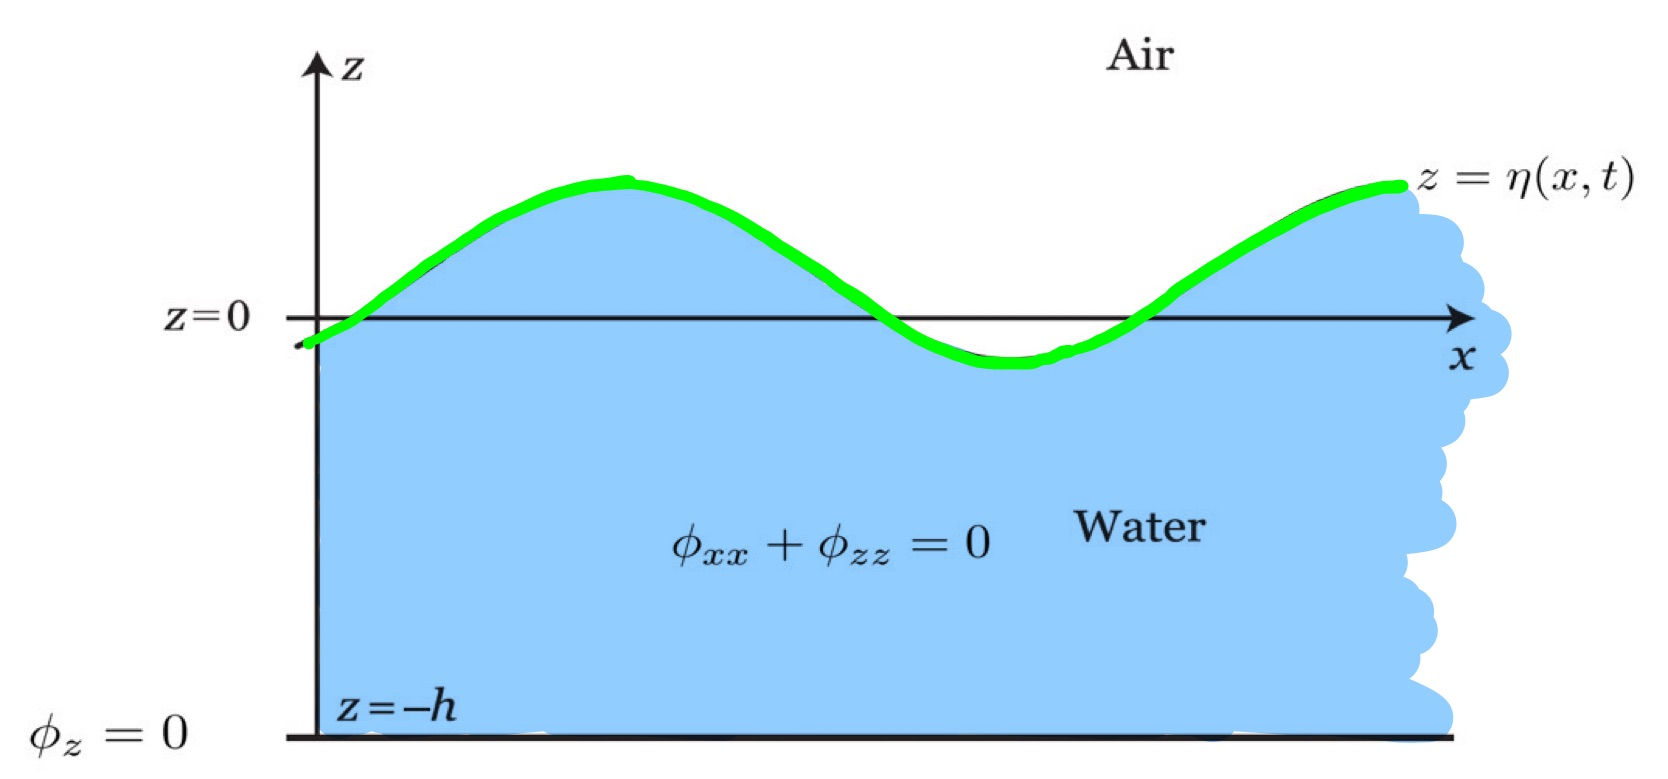
\includegraphics[scale=0.20]{Figures/FWWP.jpg}
        \caption{Physics of the full water wave problem}
        \label{fig:FWWP}
\end{center}
\end{figure}
\rmk{The reader should be aware that surface tension is made negligible in \eqref{WLP1D}. The extension of the dynamic condition \eqref{1BC2} that accommodates the effects of surface tension is 
\[ 
\phi_t + \frac{1}{2} (\phi_x^2 + \phi_z^2) + g\eta = \frac{\sigma}{\rho_0} \frac{\eta_{xx}}{(1+\eta_x^2)^{3/2}} \qquad z = \eta(x, t),
\]
where $\sigma$ is the coefficient of surface tension.}
\rmk{The way we expressed the water wave problem is in terms of the scalar field $\phi.$ Now, recall that $\V = \nabla \phi,$ where $\V$ is the velocity field of the fluid. Since $\phi$ is a potential of $\V,$ we refer to $\phi$ as the \textit{velocity potential}, and the formulations \eqref{WLP2D} and \eqref{WLP1D} are called the velocity potential formulation of the water wave problem. There is also an integral formulation of the problem that we will discuss later.}

\subsubsection{Dispersion relation}
We examine the dispersion relation. The examination is required, as dispersion relation expresses how the wave velocity depends on the wavelength. This is important in derivation of shallow-water model, where we would like the fluid to have an appropriate phase velocity. We are looking for solutions of the form 
\[\phi = A(k,t)e^{ikx} + \mathcal{O}(\epsilon^2), \eta = \bar{\eta}e^{ikx} + \mathcal{O}(\epsilon^2), \textrm{ where } A, \bar{\eta} \sim \mathcal(O)(\epsilon). \]

First, we linearise the dynamical and kinematic boundary conditions \eqref{1BC2}, \eqref{1BC3}. Let 
\[ \eta = \epsilon \eta_1 + \epsilon^2 \eta_2 + \mathcal{O}(\epsilon^3) \qquad \phi = \epsilon \phi_1 + \epsilon^2\phi_2 + \mathcal{O}(\epsilon^3) \]
where $\epsilon$ is a small parameter. Examine the terms in \eqref{1BC2}:
\[
\phi_z^2 \Big\vert_{z= \eta} = \epsilon^2 (\phi_1)_z^2 + \mathcal{O}(\epsilon^3), \quad \textrm{ and } \quad \phi_x^2 \Big\vert_{z= \eta} = \epsilon^2 (\phi_1)_x^2 + \mathcal{O}(\epsilon^3).
\]
Thus, 
\begin{align*}
\phi_t + \frac{1}{2} (\phi_{x}^2 + \phi_{z}^2) + g \eta &= 0, \qquad &z&= \eta(x,t), \\
\implies \epsilon(\phi_1)_t + \epsilon^2 (\phi_2)_t + g(\epsilon\eta_1 + \epsilon^2\eta_2) + \frac{\epsilon^2}{2}\left((\phi_1)_x^2 + (\phi_1)_z^2 \right) &= 0, \qquad &z&=0, \\
\implies \epsilon^1: \qquad \frac{\partial \phi_1}{\partial t} &= - g \eta_1, \qquad &z&= 0.
\end{align*}
Similarly, for terms in \eqref{1BC3}, we have 
\begin{align*}
\eta_t + \phi_x\eta_x &= \phi_z, \qquad &z&= \eta(x,t), \\
\implies \eta_t + \phi_x\eta_x+ \eta \frac{\partial}{\partial z}\left[ \eta_t + \phi_x\eta_x \right] &= \frac{\partial}{\partial z}\left[ \phi + \eta \phi_z \right], \qquad &z&= 0, \\
\implies \epsilon\frac{\partial \eta_1}{\partial t} + \epsilon^2\frac{\partial \eta_2}{\partial t} + \epsilon^2\frac{\partial \phi_1}{\partial x} \frac{\partial \eta_1}{\partial x}  &= \epsilon\frac{\partial \phi_1}{\partial z} + \epsilon^2 \frac{\partial \phi_2}{\partial z} + \epsilon^2 \eta_1 \frac{\partial^2 \phi_1}{\partial z^2} + \mathcal{O}(\epsilon^3), \qquad &z&= 0,\\
\implies \epsilon^1: \qquad \frac{\partial \eta_1}{\partial t}  &= \frac{\partial \phi_1}{\partial z}, \qquad &z&= 0.
\end{align*}
In sum, the boundary conditions at $z = \eta$ turn into 
\begin{equation}\label{linearisedBCs}
\frac{\partial \eta_1}{\partial t} = \frac{\partial \phi_1}{\partial z}, \qquad \frac{\partial \phi_1}{\partial t} = - g \eta_1, \qquad z=0.
\end{equation}

Next, consider a plane wave form of a solution: 
\begin{equation}\label{ExpA}
 \phi_1(x,z,t) = A(k,z,t)\exp(ikx),
\end{equation}
where $k \in \RR.$ Substituting into the PDE \eqref{1PDE}, we obtain an ODE for the amplitude:
\[ A_{zz} - k^2 A = 0, \]
whose general solution is
\[ A = \bar{A}(k,t)\cosh(k(z+h))) + \bar{B}(k,t)\sinh(k(z+h)). \]
Applying \eqref{1BC1}, we obtain that 
\[ 
A_z= 0, \qquad z = -h,
\]
which immediately implies that $\bar{B}=0.$
Assume that the free surface is of the form
\begin{equation}\label{ExpN}
\eta_1(x,t) = \bar{\eta}(k,t) \exp(ikx).
\end{equation}
Substituting \eqref{ExpA} and \eqref{ExpN} into equations in \eqref{linearisedBCs} and evaluating at $z=0$, we obtain 
\begin{align}
\frac{\partial \bar{A}}{\partial t} \cosh(kh) + g\bar{\eta_1} = 0, \label{linBCs1}\\ 
\frac{\partial \bar{\eta_1}}{\partial t} - k \sinh(kh)\bar{A}  = 0.  \label{linBCs2}
\end{align}
Take the time derivative of \eqref{linBCs2} and substitute into \eqref{linBCs1}:
\[ 
\frac{\partial^2 \bar{\eta}}{\partial t^2} +g k \tanh(kh)\bar{\eta} = 0.
\]
Further assuming that $\bar{\eta}(k,t) = \bar{\eta}(k,0)e^{-i \omega t},$ we finally derive the dispersion relation:
\begin{equation}\label{DispRel1}
\omega^2 = gk \tanh(kh).
\end{equation}
In short, we assumed that 
\[ 
\phi_1 = A(k,z,t)\exp(ikx), \qquad \eta_1(x,t) = \bar{\eta}(k,0)\exp(i(kx-\omega t)),
\]
i.e. we expressed the velocity potential and a free surface in the frequency domain, and found an expression \eqref{DispRel1} that relates a frequency $\omega$ to a wave number $k.$
Although the equation \eqref{DispRel1} has several interesting limits, we focus on the shallow-water dispersion, which occurs when $kh \ll 1.$ In this case, 
\begin{equation}\label{DispRel2}
\omega^2 = gk (kh - \frac{(kh)^3}{3} + \ldots),
\end{equation}
and in the leading order, 
\begin{equation}\label{DispRel3}
\omega^2  \approx ghk^2,
\end{equation}
so that $\omega_{\pm} \approx \pm\sqrt{gh} |k| =: \pm c_0 |k|.$ It should be clear that since $\omega$ is a wavelength, and $k$ is a wave number, $c_0 = \sqrt{gh}$ is the phase velocity of the shallow water wave. 

For convenience, we illustrate the findings visually in Figures \ref{fig:dispersiongeneral} and \ref{fig:dispersionclose}. For convenience, we let $g , h = 1,$ and in this case, we chose $k \in [0, 0.06]$ to correspond to $\sqrt{gh} \ll 1.$ As is seen, plots of \eqref{DispRel1}, \eqref{DispRel2}, and \eqref{DispRel3} are approximately the same in the green region $\sqrt{gh} \ll 1.$ Then, in this region(or more precisely, in this limit), the frequency of a shallow water wave is $\pm\sqrt{gh} |k|,$ and the velocity is $\sqrt{gh}.$
\begin{figure}
\centering
\begin{minipage}{.5\textwidth}
  \centering
  \includegraphics[width=\linewidth]{Figures/Dispersion1.pdf}
  \captionof{figure}{Dispersion on $k \in [0,2]$}
  \label{fig:dispersiongeneral}
\end{minipage}%
\begin{minipage}{.5\textwidth}
  \centering
  \includegraphics[width=\linewidth]{Figures/Dispersion2.pdf}
  \captionof{figure}{A closer look at dispersion, for $k \in [0,0.5].$}
  \label{fig:dispersionclose}
\end{minipage}
\end{figure}

\subsubsection{Nondimensionalisation}
Having expressed the problem in the velocity potential, we'd like to remove the dimensional variables. Since dimensions of the problem are directly related to the units of variables (wavelength, time, height), it is hard to decide which terms are negligible when performing an approximation procedure. Thus, we'd like to remove the dimensions of the problem, and work with ``pure'' numbers.  Define new dimensionless variables as follows:
\[ 
z = h z' \qquad x = \lambda_x x' \qquad t = \frac{\lambda_x}{c_0} t' \qquad \eta = a \eta' \qquad \phi  = \frac{\lambda_x ga}{c_0} \phi',
\]
where $c_0 = \sqrt{gh}$ is the speed of shallow water waves, $\lambda_x$ is a typical wavelength of the initial data, and $a$ is the maximum amplitude of the initial data. Note that primed variables are dimensionless. Observe that we chose new variables so that, when transformed, the problem is ``normalised" in the shallow water-wave limit. In addition, it should be clear why we divide by $c_0:$ indeed, $c_0$ is a ``typical" speed of shallow water-waves, as we found in the preceding section.

Transform the problem via chain rule (details are in the Appendix), and define dimensionless parameters $\varepsilon = a/h$ and $\mu = h/\lambda_x;$ physically, $\varepsilon$ is a measure of amplitude of the wave, and $\mu$ is a measure of the depth relative to the typical wavelength. Alternatively, $\varepsilon$ is a measure of nonlinearity, and $\mu$ is a measure of dispersion. Bringing all together and dropping the primed notation, we obtain a non-dimensionalised problem:
\begin{subequations}\label{WLP1DND1}
\begin{align}
\label{1PDEND1}  \mu^2 \phi_{xx} + \phi_{zz} &= 0 &-1 <&z < \varepsilon\eta \\
\label{1BC1ND1} \phi_z &= 0 &z &= -1  \\ 
\label{1BC2ND1} \phi_{t} + \frac{\varepsilon}{2} \left(\phi_{x}^2 + \frac{1}{\mu^2}\phi_{z}^2\right) + \eta &= 0 &z &= \varepsilon\eta(x,t)\\
\label{1BC3ND1} \mu^2 \left[\eta_{t} + \varepsilon \phi_{x} \eta_{x}\right] &= \phi_{z} &z &= \varepsilon\eta(x,t).
\end{align}
\end{subequations}
with the condition that $\phi$ tends to equilibrium as $|x|\to \infty.$ 

\section{The whole-line problem}

In this section, we derive wave and Korteweg de Vries (KdV) equations on the whole line. First, we make assumptions about the relations between $\varepsilon$ and $\mu.$ We consider long waves in shallow water, which means that the depth $h$ is small relative to the wave wavelength $\lambda_x,$ i.e.
\[ \mu = \dfrac{h}{\la_x} \ll 1.\]
Further, suppose that waves have small amplitude, so 
\[ \varepsilon = \frac{a}{h} \ll 1. \]
Now, by Kruskal's principle of maximal balance, to obtain equations that are interesting, we should balance all of these assumptions by connecting them to each other. For this derivation, we choose $\varepsilon = \mu^2.$ This is to reflect the balance of ``weak nonlinearity'' and ``weak dispersion''. However, there is no reason not to balance in other ways, say $\varepsilon = \sqrt{\mu}.$ There are many options, and some of them will give interesting equations, while others will not lead to anything. As such, it is this assumption in our procedure that determines the relevance of to-be-derived equations. Thus, the nondimensional problem \eqref{WLP1DND1} becomes:
\begin{subequations}\label{WLP1DND2}
\begin{align}
\label{1PDEND2}  \varepsilon\phi_{xx} + \phi_{zz} &= 0 &-1 <&z < \varepsilon\eta \\
\label{1BC1ND2} \phi_z &= 0 &z &= -1  \\ 
\label{1BC2ND2} \phi_{t} + \frac{1}{2} \left(\varepsilon\phi_{x}^2 + \phi_{z}^2\right) + \eta &= 0 &z &= \varepsilon\eta(x,t)\\
\label{1BC3ND2} \varepsilon\left[\eta_{t} + \varepsilon \phi_{x} \eta_{x}\right] &= \phi_{z} &z &= \varepsilon\eta(x,t).
\end{align}
\end{subequations}
with the condition that $\phi$ is in equilibrium as $|x|\to \infty.$

\subsection{Derivation of Wave \& KdV equations}

\subsubsection{Via velocity potential formulation}
We are now ready to perform an approximation procedure. We produce the derivation in the way as given in \cite[Chapter 4]{bernard}. Note that there is another derivation, given in \cite[Chapter 5]{ablowitz}. First, we determine the dependence on $z.$ Assume the expansion 
\[
\phi(x,z,t) = \phi_0(x,z,t) + \epsilon \phi_1(x,z,t) + \epsilon^2 \phi_2(x,z,t) + \ldots
\]
Substituting the expansion into \eqref{1PDEND2}, we obtain
\begin{align*}
0 = \epsilon\phi_{xx} + \phi_{zz} &= \epsilon\phi_{0xx} + \epsilon^2 \phi_{1xx}+ \epsilon^3 \phi_{2xx} + \phi_{0zz} + \epsilon \phi_{1zz}+ \epsilon^2 \phi_{2zz} + \ldots \\
&= \phi_{0zz} + \epsilon(\phi_{0xx} + \phi_{1zz}) + \epsilon^2(\phi_{1xx}+\phi_{2zz}) + \ldots
\end{align*}
so that in powers of $\epsilon,$ we have
\begin{align*}
&\epsilon^0: &\phi_{0zz} &= 0 &&\implies \phi_0 = \phi_0(x,t), \\
&\epsilon^1: &\phi_{0xx} + \phi_{1zz} &= 0 &&\implies \phi_1 = - \phi_{0xx} \frac{(z+1)^2}{2},\\
&\epsilon^2: &\phi_{1xx}+\phi_{2zz} &= 0 &&\implies \phi_2 = \phi_{0xxxx} \frac{(z+1)^4}{4!},
\end{align*}
and so forth. Thus, the general solution to \eqref{1PDEND1} and \eqref{1BC1ND2} is 
\begin{equation}\label{ExpansionPhi}
\phi(x,z,t) = \phi_0 - \epsilon\frac{(z+1)^2}{2!}\phi_{0xx} + \epsilon^2 \frac{(z+1)^4}{4!}\phi_{0xxxx} - \ldots = \sum^{\infty}_{k=0} (-1)^k \epsilon^k \frac{(z+1)^{2k}}{(2k)!} \partial^k_x \phi_0.
\end{equation}

\subsubsection*{Leading order approximation}
Now, we find the leading order terms in \eqref{1BC2ND2} and \eqref{1BC3ND2}:
\begin{align*}
\phi_{t} + \frac{1}{2} \left(\varepsilon\phi_{x}^2 + \phi_{z}^2\right) + \eta &= 0 &z &= \varepsilon\eta(x,t)\\
\varepsilon\left[\eta_{t} + \varepsilon \phi_{x} \eta_{x}\right] &= \phi_{z} &z &= \varepsilon\eta(x,t).
\end{align*}
Substituting \eqref{ExpansionPhi} into a kinematic condition and evaluating at $z = \varepsilon \eta$ yields 
\[
\phi_z  = -\varepsilon(\varepsilon \eta + 1) \phi_{0xx} + \ldots = -\varepsilon \phi_{0xx} + \ldots,
\]
so that 
\begin{align*}
\varepsilon\left[\eta_{t} + \varepsilon \phi_{x} \eta_{x}\right] = \phi_{z} \qquad \implies \qquad \varepsilon \eta_{t} = -\epsilon \phi_{0xx} \qquad \implies \qquad  \eta_{t}  +  (\phi_{0x})_x &= \mathcal{O}(\varepsilon),
\end{align*}
where we ignored all terms of order at least $\varepsilon^2.$ As for the dynamic condition, note that at $z = \varepsilon \eta,$ we have 
\[ \varepsilon\phi_x^2  \sim \mathcal{O}(\epsilon), \qquad \phi_z^2 \sim \mathcal{O}(\epsilon^2), \qquad \phi_t = \phi_{0t} + \mathcal{O}(\epsilon),\]
so that 
\begin{align*}
\phi_{t} + \frac{1}{2} \left(\varepsilon\phi_{x}^2 + \phi_{z}^2\right) + \eta = 0 \qquad \implies \qquad \phi_{0t} + \eta = \mathcal{O}(\epsilon) \qquad \implies \qquad (\phi_{0x})_t + \eta_x &= \mathcal{O}(\varepsilon),
\end{align*}
where in the last equation we took a partial derivative in $x$ and interchanged in the term $\phi_{0x}.$ In sum, we obtained
\begin{subequations} \label{1stOrdP}
\begin{align}
\eta_{t}  +  (\phi_{0x})_x &= \mathcal{O}(\varepsilon), \\
(\phi_{0x})_t + \eta_x &= \mathcal{O}(\varepsilon).
\end{align}
\end{subequations}

Our goal is to determine $\phi_{0x}$ and $\eta.$ Observe that, however, the equations are inhomogeneous, and so, the best we can hope for, is an approximation for $\phi_{0x}$ and $\eta.$ Therefore, we introduce perturbation expansions
\begin{subequations} \label{PertExpns}
\begin{align}
\phi_{0x} &= u_0 + \epsilon u_1 + \epsilon^2 u_2 + \mathcal{O}(\epsilon^3) \\
\eta &= \eta_0 + \epsilon \eta_1 + \epsilon^2 \eta_2 + \mathcal{O}(\epsilon^3).
\end{align}
\end{subequations}
Further, we introduce slow time scales 
\[ 
\tau_0 = t, \qquad \tau_1 = \epsilon t, \qquad \tau_2 = \epsilon^2 t, \qquad \tau_j = \epsilon^j t, \quad j = 0,1,2,  \ldots
\]
so that 
\begin{equation}\label{TimeScales}
\frac{\partial}{\partial t} = \frac{\partial}{\partial \tau_0} +  \epsilon\frac{\partial}{\partial \tau_1} + \epsilon^2 \frac{\partial}{\partial \tau_2} + \mathcal{O}(\epsilon^3). 
\end{equation}
See Remark 3 for an explanation for the multiple times scales. We are ready to derive the equations. Applying the expansions \eqref{PertExpns} and \eqref{TimeScales} to LHS of \eqref{1stOrdP}, we have
\begin{align*}
\eta_{t} + (\phi_{0x})_x &= \eta_{0t} + u_{0x} + \epsilon (\eta_{1t}+ u_{1x}) + \mathcal{O}(\epsilon^2) \\
&= \eta_{0\tau_0} + u_{0x} + \epsilon \eta_{0\tau_1} + \mathcal{O}(\epsilon) \\
&= \eta_{0\tau_0} + u_{0x} + \mathcal{O}(\epsilon), \\
\intertext{ and }
(\phi_{0x})_t + \eta_x &= (u_0 + \epsilon u_1)_t + \eta_{0x} + \epsilon \eta_{1x} + \mathcal{O}(\epsilon^2) \\
&= u_{0t} + \eta_{0x} + \mathcal{O}(\epsilon) \\
&= u_{0\tau_0} + \eta_{0x} + \mathcal{O}(\epsilon).
\end{align*}
Thus, at the lowest order, we have
\begin{align*}
\eta_{t}  +  (\phi_{0x})_x &= \mathcal{O}(\varepsilon) \implies u_{0\tau_0} + \eta_{0x} + \mathcal{O}(\epsilon)= \mathcal{O}(\varepsilon) \implies u_{0\tau_0} + \eta_{0x} = 0, \\
(\phi_{0x})_t + \eta_x &= \mathcal{O}(\varepsilon) \implies u_{0\tau_0} + \eta_{0x} + \mathcal{O}(\epsilon) = \mathcal{O}(\epsilon) \implies u_{0\tau_0} + \eta_{0x} = 0.
\end{align*}
Decoupling these equations, we obtain two \textbf{wave} equations with velocity 1, in variables $x$ and $\tau_0,$
\begin{align*}
\frac{\partial^2 \eta_{0}}{\partial \tau_0^2} - \frac{\partial^2\eta_{0}}{\partial x^2} = 0, \qquad \frac{\partial^2 u_{0}}{\partial \tau_0^2} - \frac{\partial^2 u_{0}}{\partial x^2} = 0.
\end{align*}
Thus, the general solutions are
\begin{align*}
\eta_{0}(x, \tau_0, \tau_1, \ldots) &= f(x- \tau_0, \tau_1, \ldots) + g(x+ \tau_0, \tau_1, \ldots), \\
u_{0}(x, \tau_0, \tau_1, \ldots) &= f(x- \tau_0, \tau_1, \ldots) - g(x+ \tau_0, \tau_1, \ldots).
\end{align*}
Physically, on the fastest time scale $\tau_0,$ the surface and velocity potential are described by left-going and right-going waves. Note that the above expressions are general solutions, and, to obtain more meaningful solutions, we determine what exactly $f$ and $g$ are. Initial conditions by themselves are not enough, for they do not explain the behaviour of $f,g$ on the next time scale $\tau_1.$ For example, there might be some effects that are not present at $\tau_0$ but lead to blowing up at $\tau_1.$ Determining the dependence on $\tau_1$ will enable us to understand such effects. This is done in the next order equations.

\subsubsection*{Determining $f,g$}
Recall equations \eqref{1BC2ND2} and \eqref{1BC3ND2}:
\begin{align*}
\phi_{t} + \frac{1}{2} \left(\varepsilon\phi_{x}^2 + \phi_{z}^2\right) + \eta &= 0, &z &= \varepsilon\eta(x,t),\\
\varepsilon\left[\eta_{t} + \varepsilon \phi_{x} \eta_{x}\right] &= \phi_{z}, &z &= \varepsilon\eta(x,t).
\end{align*}
Using the expansion \eqref{ExpansionPhi} for $\phi,$ perturbation expansions \eqref{PertExpns}, and multiple time scales \eqref{TimeScales}, we obtain the relevant terms:
\begin{align*}
\phi_z(x, \epsilon \eta(x,t), t) &= -\epsilon u_{0x} + \epsilon^2 \left(-\eta_0 u_{0x} - u_{1x} + \frac{1}{6}u_{0xxx} \right) + \mathcal{O}(\epsilon^3), \\
\phi_x(x, \epsilon \eta(x,t), t) &= u_0 + \epsilon(u_1 - \frac{1}{2}u_{0xx}) + \mathcal{O}(\epsilon^2), \\
\phi_{xt}(x, \epsilon \eta(x,t), t) &=u_{0\tau_0} + \epsilon(u_{0\tau_1} + u_{1\tau_0} - \frac{1}{2}u_{0xx\tau_0})+ \mathcal{O}(\epsilon^2), \\
\eta_t &= \eta_{0\tau_0} + \epsilon(\eta_{1\tau_0} + \eta_{0\tau_1}) + \mathcal{O}(\epsilon^2).
\end{align*}
Thus, the dynamic condition, in powers of $\epsilon,$ becomes: 
\begin{align*}
&\epsilon^0: &\eta_{0\tau_0} + u_{0x} &= 0, \\
&\epsilon^1: &\eta_{1\tau_0} + u_{1x} &= - (u_{0\tau_1} -\frac{1}{2} u_{0xx\tau_0} + u_0 u_{0x}). 
\end{align*}
The kinematic condition, in powers of $\epsilon,$ can be rewritten as:
\begin{align*}
&\epsilon^1: &\eta_{0\tau_0} + u_{0x} &= 0, \\
&\epsilon^2: &\eta_{1\tau_0} + u_{1x} &= - (\eta_{0\tau_1} + u_0 \eta_{0x} + \eta_0 u_{0x} - \frac{1}{6}u_{0xxx}).
\end{align*}
As expected, in lowest order, we obtain equations that can be decoupled into wave equations. In the next order, we obtain
\begin{subequations}\label{2ndOrdP}
\begin{align}
\eta_{1\tau_0} + u_{1x} &= - (\eta_{0\tau_1} + u_0 \eta_{0x} + \eta_0 u_{0x} - \frac{1}{6}u_{0xxx}), \label{2ndOrdP1} \\
\eta_{1\tau_0} + u_{1x} &= - (u_{0\tau_1} -\frac{1}{2} u_{0xx\tau_0} + u_0 u_{0x}). \label{2ndOrdP2}
\end{align}
\end{subequations}
Observe that the RHS of \eqref{2ndOrdP} are functions $u_0, \eta_0,$ whose general form we know. Now, we can determine the relationship between $u_0, \eta_0$ and $\tau_1;$ this will enable us to derive a more meaningful form for $u_0, \eta_0.$ It is worth pointing out that in what follows, we may also determine how $u_1, \eta_1$ depend on $\tau_1,$ but we will not need this information, for we are only interested in the leading order approximation.

Given the equations, we can decouple them via characteristic variables:
\begin{equation}\label{CharVars}
l = x + \tau_0, \qquad r= x - \tau_0.
\end{equation}
In this case, $l$ is the characteristic variable for a left-going wave, and $r$ is the characteristic variable for a right-going wave. Then, 
\[ 
\partial_x = \partial_r + \partial_l, \qquad \partial_{\tau_0} = \partial_l - \partial_r.
\]
Therefore, we have $\eta_0 = f(r) + g(l), u_0 = f(r)- g(l).$ Substituting these expressions into \eqref{2ndOrdP}, we obtain:
\begin{align*}
\eta_{1l} - \eta_{1r} + u_{1r} + u_{1l} &= - (-f_{\tau_1} - g_{\tau_1} + (f-g)(f_r + g_r) + (f + g)(f_r- g_l) - \frac{1}{6}(f_{rrr}-g_{lll})), \\
u_{1l} - u_{1r} + \eta_{1r} + \eta_{1l} &= - (f_{\tau_1} - g_{\tau_1} + (f-g)(f_r - g_l) - \frac{1}{2}(f_{rrr}+g_{lll})).
\end{align*}
Adding and subtracting resulting equations yields:
\begin{align*}
2(\eta_{1l} + u_{1l}) &= - (2f_{\tau_1}+ 3ff_r + \frac{1}{3}f_{rrr}) +f_r g +g g_l + fg_l - \frac{2}{3}g_{lll}, \\
2(u_{1r} - \eta_{1r}) &= - (2g_{\tau_1} - 3gg_l - \frac{1}{3}g_{lll}) - g_l f- f f_r - g f_r + \frac{2}{3}f_{rrr}. 
\end{align*}
Integration of LHS produces:
\begin{subequations}\label{2ndOrdPF}
\begin{align}
2(\eta_{1} + u_{1}) &= - (2f_{\tau_1}+ 3ff_r + \frac{1}{3}f_{rrr})l +f_r \int g \D l +\frac{1}{2}g^2 + fg - \frac{2}{3}g_{ll} + C_1, \\
2(u_{1} - \eta_{1}) &= - (2g_{\tau_1} - 3gg_l - \frac{1}{3}g_{lll})r - g_l \int f \D - \frac{1}{2}f^2 - g f + \frac{2}{3}f_{rr} + C_2,
\end{align}
\end{subequations}
Terms on LHS of \eqref{2ndOrdPF} are clearly bounded. Thus, all the terms on RHS of both equations must be bounded, except for the first terms (they grow without bound), and second ones. We may assume that profiles under consideration are the ones where the left- and right-translating frames do not interact, so that the integrals vanish. In addition, since terms on LHS are bounded, the growth of first terms is unphysical. Thus, we impose that 
\[ 
2f_{\tau_1}+ 3ff_r + \frac{1}{3}f_{rrr} = 0, \qquad 2g_{\tau_1} - 3gg_l - \frac{1}{3}g_{lll} = 0.
\]
We have thus derived two KdV equations on the whole line. Note that this model is valid in frames moving with a shallow water velocity, and after sufficient time has elapsed so that right- and left-moving waves do not interact. Solving for $f, g$ along with appropriate initial data, yields a leading order approximation for the velocity potential $u_0$ and free surface $\eta_0:$
\begin{subequations}\label{GenSoln1}
\begin{align}
\eta_{0} &= f(x- \tau_0, \tau_1, \ldots) + g(x+ \tau_0, \tau_1, \ldots), \\
u_{0} &= f(x- \tau_0, \tau_1, \ldots) - g(x+ \tau_0, \tau_1, \ldots),
\end{align}
\end{subequations}
where $f,g$ solve the above KdV equations. In particular, if our data is 
\[ \eta(x,0) = V(x), \qquad \phi(x,\eta, 0)= U(x),\]
then the appropriate data for $f,g$ is given by:
\begin{align*}
V(x) \approx  \eta_0(x, 0) = f(x - 0, 0, \ldots) + g(x+0, 0, \ldots), \\
U(x) \approx u_{0}(x, \eta, 0) = f(x- 0, 0, \ldots) - g(x+ 0, 0, \ldots),
\end{align*}
so that adding and subtracting two equations yields initial conditions for $f,g:$
\begin{align*}
V(x) + U(x) =2 f(x - 0, 0, \ldots), \\
U(x) - V(X) = 2g(x+ 0, 0, \ldots).
\end{align*}

\rmk{The introduction of perturbation expansions \eqref{PertExpns} is justified easily, but that of time scales \eqref{TimeScales} is not as intuitive. One could say that physically, time scales allow us to separate the different time dynamics that can be present in a physical phenomenon. However, what is a mathematical explanation? For now, we will just say it works; in the next report, we aim to demonstrate that if time scales are not used, the solutions will be secular.
}
\rmk{One question that might arise is: how can we justify the conclusion, i.e. how can we know that $f,g$ really approximate $\eta$ and $\phi$ in the leading order? At this point, our response is that all we did is a formal expansion. We will justify the expansion numerically and analytically in the second half of the project, which may involve estimating error, calculating stability and convergence, and more.}
\section{The half-line problem}
The original 4 equations \eqref{1PDE}, \eqref{1BC1}, \eqref{1BC2}, \eqref{1BC3} remain the same. We change \eqref{1BC4} and add that  two more conditions on $\phi$ and $\eta$ at $x=0,$ so that our new system is:
\begin{subequations} \label{DimHalfLineProblem}
\begin{align}
\phi_{xx} + \phi_{zz} &= 0, &-h < z < \eta(x,t), \\
\phi_{z} &= 0, &z = -h, \\
\label{BC1}\phi_{x} &= 0, &x =0, \\
\eta_t + \phi_{x}\eta_{x} &= \phi_{z}, & z = \eta(x,t), \\
\phi_t + g\eta + \frac{1}{2}(\phi_{x}^2 + \phi_{z}^2) &= 0, &z = \eta(x,t), \\
\label{BC2} \phi_{z}(0,\eta,t) &= \eta_t(0,t), &(x,z) = (0,\eta). \\
\label{BC3} |\phi| \to 0, |\eta| &\to 0,  &x &\to \infty,
\end{align}
\end{subequations}

Physically, we put up a barrier at $x=0$ such an impenetrable tall wall, so that all water is flowing to the right. This is illustrated by Figure \ref{fig:HWWP}:
\begin{figure}[h]
\begin{center}
        \includegraphics[scale=0.15]{Figures/HWWP.jpg}
        \caption{Physics of the half-line water wave problem}
        \label{fig:HWWP}
\end{center}
\end{figure}

The dispersion relation for this problem is the same as that for the whole-line problem. Thus, we introduce the same nondimensional variables; the first 4 equations transform as before. The non-dimensional problem becomes:
\begin{subequations} \label{NondimHalfLineProblem}
\begin{align}
\label{NondimPDE}\epsilon\phi_{xx} + \phi_{zz} &= 0, &-1 < z < \epsilon\eta, \\
\label{NondimBC1}\phi_{z} &= 0, &z = -1, \\
\label{NondimBC2}\phi_{x} &= 0, &x =0, \\
\label{NondimBC3}\epsilon\eta_t + \epsilon^2 \phi_{x}\eta_{x} &= \phi_{z}, & z = \epsilon\eta,\\
\label{NondimBC4}\phi_t + \eta + \frac{1}{2}(\epsilon\phi_{x}^2 + \phi_{z}^2) &= 0, &z = \epsilon\eta, \\
\label{NondimBC5}\phi_{z}(0,\epsilon\eta,t) &= \epsilon\eta_t(0,t), &(x,z) = (0,\epsilon\eta), \\
\label{NondimBC6} |\phi| \to 0, |\eta| &\to 0,  &x &\to \infty.
\end{align}
\end{subequations}

\rmk{As we will see later, equation \eqref{NondimBC2} will impact the approximation procedure. On the other hand, the equations \eqref{NondimBC5} and \eqref{NondimBC3}, when expanded, are identical in the leading order, except that the latter is to be satisfied at $x = 0.$ Thus, there is no need to work with \eqref{NondimBC5}, since \eqref{NondimBC3} captures the same behaviour. In turn, this begs a question: why we do impose this condition? For now, the answer is that we need to impose the physical conditions of the problem, and we think that this might be the one. Clearly, this explanation is not a clear-cut way to determine an appropriate condition, but, as will be seen later, it is not easy to determine the relevant condition. Determining the condition will be closely investigated in December, and results will be reported in Semester 2.}

\subsection{Derivation of Wave \& KdV equations}

\subsubsection{Via velocity potential formulation}
We tentatively derive the KdV equations on a half-line. The same procedure is largely the same as in the previous section; thus, we only comment where the derivation differs from the whole line case. We know that the expansion \eqref{ExpansionPhi} satisfies \eqref{NondimPDE} and \eqref{NondimBC1}. Applying the condition \eqref{NondimBC2}, we obtain the following expansion:
\begin{equation}\label{ExpansionPhi2}
\phi(x,z,t) = \phi_0 - \epsilon\frac{(z+1)^2}{2!}\phi_{0xx} + \epsilon^2 \frac{(z+1)^4}{4!}\phi_{0xxxx} - \ldots \qquad \partial_x^{2k+1}\phi_0(0,t) = 0 ~\forall k \in \NN.
\end{equation}
Expanding the kinematic and dynamic conditions, we obtain the following equations:
\begin{subequations} \label{NonDimHalfLineProb1}
\begin{align}
\label{P1BC1}\eta_t + \partial_x\phi_{0x} &= \mathcal{O}(\epsilon), &z &= \epsilon\eta, \\
\label{P1BC2}\partial_t\phi_{0x} + \partial_x \eta &=  \mathcal{O}(\epsilon), &z &= \epsilon\eta,  \\
\label{P1BC3}\eta_t + \partial_x\phi_{0x} &= \mathcal{O}(\epsilon), &(x,z) &= (0,\epsilon\eta), \\
\label{P1BC4}\phi_{0x} &= 0, &x &= 0,
\end{align}
\end{subequations}
where \eqref{P1BC4} follows from \eqref{ExpansionPhi2}. We can merge \eqref{P1BC3} and \eqref{P1BC1} into one equation, since they are essentially the same equation. Introducing the perturbation expansions \eqref{PertExpns}, time scales \eqref{TimeScales}, we obtain a leading order problem
\begin{subequations} \label{NonDimHalfLineProb2}
\begin{align}
\label{P2BC1}\eta_{0\tau_0} + u_{0x} &=0, &z &= \epsilon\eta, x \geq 0, \\
\label{P2BC2} u_{0\tau_0} + \eta_{0x} &= 0, &z &= \epsilon\eta,  \\
\label{P2BC3} u_0 &= 0, &x &= 0.
\end{align}
\end{subequations}
The problem \eqref{NonDimHalfLineProb2} then yields:
\begin{align*}
\frac{\partial^2 \eta_0}{\partial \tau_0^2} - \frac{\partial^2 \eta_0}{\partial x^2} = 0, \qquad \frac{\partial^2 u_0}{\partial \tau_0^2} - \frac{\partial^2 u_0}{\partial x^2} = 0, \qquad x\geq0, \qquad z= \epsilon \eta,
\end{align*}
along with a boundary condition $u_0 = 0$ at $x=0.$ We thus have a boundary value problem for $u_0,$ i.e. one of solving a wave equation with a semi-infinite fixed end, which has piecewise solutions:
\begin{align*}
u_0 = \begin{cases} F(x - \tau_0, \tau_1, \ldots) + G(x+\tau_0, \tau_1, \ldots) & x>\tau_0 \\ -G(\tau_0 - x,  \tau_1, \ldots) + G(x+\tau_0,  \tau_1, \ldots) & x< \tau_0 \end{cases},
\end{align*}
which follows since $F,G$ are defined on $[0, \infty).$ Since $u_0$ and $\eta_0$ are related by \eqref{P2BC1} and \eqref{P2BC2}, it follows that
\begin{align*}
\eta_0 = \begin{cases} F(x - \tau_0,  \tau_1, \ldots) - G(x+\tau_0,  \tau_1, \ldots) & x>\tau_0 \\ -G(\tau_0 - x,  \tau_1, \ldots) - G(x+\tau_0,  \tau_1, \ldots) & x< \tau_0 \end{cases}.
\end{align*}
The solutions $u_0, \eta_0$ are still in general form as before in the whole line case, and so we go to the next order to obtain more meaningful results. We obtain:
\begin{align*}
\eta_{1\tau_0} + u_{1x} &= - (\eta_{0\tau_1} + u_0 \eta_{0x} + \eta_0 u_{0x} - \frac{1}{6}u_{0xxx}) \\
\eta_{1\tau_0} + \eta_{1x} &= - (u_{0\tau_1} - \frac{1}{2}u_{0xxx\tau_0} + u_0 u_{0x}),
\end{align*}
along with the boundary conditions $u_0 = u_1 = 0$ at $x = 0.$ Introduce characteristic variables, to separate the left and right going waves:
\[ 
l = x + \tau_0, \qquad r = x - \tau_0, 
\]
so that 
\[ 
\partial_x = \partial_r + \partial_l, \qquad \partial_{\tau_0} = \partial_l - \partial_r.
\]
Thus, 
\begin{align*}
u_0 = \begin{cases} F(r) + G(l) & r>0 \\ -G(-r) + G(l) =: -G(-r)+G & r<0 \end{cases} \qquad\qquad \eta_0 = \begin{cases} F(r)-G(l) & r>0 \\ -G(-r) - G(l)=: -G(-r) - G & r<0 \end{cases} 
\end{align*}
where we let $G$ be a function of $l,$ to ease the notation. Also, keep in mind that $F,G$ are also functions of $\tau_0, \tau_1, \tau_2, \ldots.$ If $r > 0,$ then the situation is identical that to the whole-line problem and we obtain the KdV equations. Thus, we deal with the case $r<0.$ For convenience, let $-r = k,$ so that $\partial_{-r} = \partial_k = - \partial_r,$ and $G(-r)= G(k).$ The transformed equations are
\begin{align*}
\eta_{1l} - \eta_{1r} + u_{1r} + u_{1l} &= - (-G(k)_{\tau_1} - G_{\tau_1} + (-G(k) + G)(G(k)_k - G_l) - (-G(k) - G)(G(k)_k + G_l)\\
&- \frac{1}{6}(G(k)_{kkk}+G_{lll})), \\
&= -(-G(k)_{\tau_1} - G_{\tau_1} - 2G(k)G(k)_k - 2G G_l - \frac{1}{6}(G(k)_{kkk}+G_{lll})), \\
\intertext{and}
u_{1l} - u_{1r} + \eta_{1r} + \eta_{1l}  &= - (-G(k)_{\tau_1} + G_{\tau_1} - \frac{1}{2}(-G(k)_{kkk} + G_{lll}) - (G(k) + G)(G(k)_k+G_l)), \\
&=  - (-G(k)_{\tau_1} + G_{\tau_1} - \frac{1}{2}(-G(k)_{kkk} + G_{lll}) - G(k)G_l - G(k)G(k)_k + G G_l+GG(k)_k).
\end{align*}
Adding and subtracting the above yields
\begin{align*}
2(\eta_{1l} + u_{1l}) &= -\left( -2G(k)_{\tau_1} - 3 G(k)G(k)_k + \frac{1}{3}G_{kkk} \right) + GG_l  - G G(k)_k + G(k)G_l + \frac{2}{3} G_{lll}, \\
2(\eta_{1k} - u_{1k}) &=  - \left(-2G_{\tau_1} - 3GG_l + \frac{1}{3}G_{lll}\right) + G(k)G(k)_k - G(k)G_l + G G(k)_k + \frac{2}{3}G(k)_{kkk}, 
\end{align*}
where we changed the derivative in LHS, using
\[ 
u_{1r} - \eta_{1r} = \partial_r (u_1 - \eta_1) = (-\partial_r)(\eta_1 - u_1) = \partial_k(\eta_1 - u_1) = \eta_{1k} - u_{1k}.
\]
Finally, we integrate the LHS, to obtain:
\begin{align*}
2(\eta_{1} + u_{1}) &= -\left(-2G(k)_{\tau_1} - 3 G(k)G(k)_k + \frac{1}{3}G_{kkk}\right)l + \frac{1}{2}G^2  - G(k)_k \int G \D l + G(k)G + \frac{2}{3} G_{ll} + C_1, \\
2(\eta_{1} - u_{1}) &=  - \left(-2G_{\tau_1} - 3GG_l + \frac{1}{3}G_{lll}\right)k + \frac{1}{2}G(k)^2 - G_l \int G(k) \D k +GG(k) + \frac{2}{3}G(k)_{kk} + C_2. 
\end{align*}
We observe that the only secular terms here are the integrals and terms that contain $k$ and $l,$ by a similar argument as in a whole line case. Thus, we require that 
\[ 
-2G(k)_{\tau_1} - 3 G(k)G(k)_k + \frac{1}{3}G_{kkk} = 0, \qquad -2G_{\tau_1} - 3GG_l + \frac{1}{3}G_{lll} = 0.
\] 
But these two equations are the same, the only difference being the variable of a function $G.$ At this point, it is not clear as to how we should interpret the terms 
\[ G(k)_k \int G \D l,  \qquad G_l \int G(k) \D k. \]
These terms might be secular, and therefore cannot be bounded a priori without additional care. This is the current topic of investigation, and will be handled with upcoming work during Semester 2. 
\section{Future directions}
In this report, we have largely focused on the classical derivation in the velocity potential. Now, our goal is to understand the non-local formulation of the problem, and attempt to rederive wave and KdV equations, from this formulation. This is intended to be done on the whole line and half line. Using our enhanced understanding of \eqref{WLP1D} from the non-local formulation, we will attempt to complete the derivation of KdV equations on the half-line. In particular, we want to understand the role of terms 
\[ G(k)_k \int G \D l,  \qquad G_l \int G(k) \D k, \]
in the half-line case, to be able to determine the appropriate KdV equation. In addition, we need to understand the type of initial conditions that the half-line problem can admit. At the same time, we will develop a better understanding of tools such as dispersion relation and examine properties of solutions via numerical simulations. 

\begin{appendices}
\subsection*{Nondimensionalisation}
We provide the details of nondimensionalisation. Define new dimensionless variables as follows:
\[ 
z = h z' \qquad x = \lambda_x x' \qquad t = \frac{\lambda_x}{c_0} t' \qquad \eta = a \eta' \qquad \phi  = \frac{\lambda_x ga}{c_0} \phi',
\]
where $c_0 = \sqrt{gh}$ is the speed of shallow water waves, $\lambda_x$ is a typical wavelength of the initial data, and $a$ is the maximum amplitude of the initial data. Note that primed variables are dimensionless. We transform the problem \eqref{WLP1D}.
First, by chain rule, we have
\[ 
\phi_{xx} = \frac{ga}{\lambda_x c_0} \phi_{x'x'}' \qquad \phi_{zz} = \frac{\lambda_x ga}{h^2c_0} \phi_{z'z'}'\] 
so that the PDE \eqref{1PDE} becomes
\[\frac{ga}{\lambda_x c_0} \phi_{x'x'}' + \frac{\lambda_x ga}{h^2c_0} \phi_{z'z'}' = 0 \implies \frac{1}{\lambda_x^2} \phi_{x'x'}' + \frac{1}{h^2} \phi_{z'z'}' = 0.
\]
The interval $z \in (h, \eta)$ becomes $hz' \in [-h, a h \eta'],$ so that $z' \in [-1, \frac{a \eta'}{h}].$ For the bottom condition \eqref{1BC1}, we have
\[ 
\phi_z =  \frac{\lambda_x ga}{h c_0} \phi_{z'}',
\]
so that 
\[ \phi_z = 0 \qquad z = - h \implies \phi_{z'}' = 0 \qquad z = -1. \]
Now, note that 
\[ 
\phi_t = ga \phi_{t'}' \qquad \phi_x^2 = \left(\frac{ga}{c_0} \phi_{x'}'\right)^2 = \left(\frac{ga}{c_0}\right)^2 \left(\phi_{x'}'\right)^2 \qquad \phi_z^2 = \left(\frac{\lambda_x ga}{hc_0}\phi_{z'}'\right)^2 = \frac{\lambda_x^2}{h^2}\left(\frac{ga}{c_0}\right)^2\left(\phi_{z'}'\right)^2 \qquad g\eta = ga\eta'
\]
so that the dynamic condition \eqref{1BC2} transforms into:
\begin{align*}
\phi_t + \frac{1}{2} (\phi_{x}^2 + \phi_{z}^2) + g \eta = 0 &\implies ga \phi_{t'}' + \frac{1}{2}\left(\frac{ga}{c_0}\right)^2 \left((\phi_{x'}')^2 + \frac{\lambda_x^2}{h^2}(\phi_{z'}')^2\right) + ga \eta' = 0 \\
&\implies \phi_{t'}' + \frac{a}{2h} \left((\phi_{x'}')^2 + \frac{\lambda_x^2}{h^2}(\phi_{z'}')^2\right) + \eta' = 0,
\end{align*}
at $z' = a\eta'/h.$ Finally, note that 
\[ 
\eta_t = \frac{ac_0}{\lambda_x}\eta_{t'}' \qquad \eta_x = \frac{a}{\lambda_x}\eta_{x'}',
\]
so that the kinematic condition \eqref{1BC3} becomes
\begin{align*}
\phi_z = \eta_t + \phi_x\eta_x &\implies \frac{\lambda_x ga}{h c_0} \phi_{z'}'=\frac{ac_0}{\lambda_x}\eta_{t'}' + \frac{ga^2}{\lambda_xc_0} \phi_{x'}' \eta_{x'}' \\
&\implies \frac{\lambda_x^2}{h^2} \phi_{z'}'= \eta_{t'}' + \frac{a}{h} \phi_{x'}' \eta_{x'}',
\end{align*}
at $z' = a\eta'/h.$ Now, define dimensionless parameters $\varepsilon = a/h$ and $\mu = h/\lambda_x;$ physically, $\varepsilon$ is a measure of amplitude of the wave, and $\mu$ is a measure of the depth relative to the typical wavelength. Alternatively, $\varepsilon$ is a measure of nonlinearity, and $\mu$ is a measure of dispersion. Bringing all together and dropping the primed notation, we obtain a non-dimensionalised problem:
\begin{subequations}\label{WLP1DND1}
\begin{align}
\label{1PDEND1}  \mu^2 \phi_{xx} + \phi_{zz} &= 0 &-1 <&z < \varepsilon\eta \\
\label{1BC1ND1} \phi_z &= 0 &z &= -1  \\ 
\label{1BC2ND1} \phi_{t} + \frac{\varepsilon}{2} \left(\phi_{x}^2 + \frac{1}{\mu^2}\phi_{z}^2\right) + \eta &= 0 &z &= \varepsilon\eta(x,t)\\
\label{1BC3ND1} \mu^2 \left[\eta_{t} + \varepsilon \phi_{x} \eta_{x}\right] &= \phi_{z} &z &= \varepsilon\eta(x,t).
\end{align}
\end{subequations}
with the condition that $\phi$ tends to equilibrium as $|x|\to \infty.$

\subsubsection*{Alternative derivation}
Another derivation is given in \cite[Chapter 5]{ablowitz}, of which we give an outline. There, one substitutes the expansion \eqref{ExpansionPhi} into the dynamic and kinematic conditions, and retains the first two leading terms to obtain
\begin{align*}
\eta &= -A_t + \frac{\epsilon}{2}(A_{xxt} - A_x^2) + \ldots, \\
\eta_t + \epsilon \eta_x A_x &= -A_{xx}(1+ \epsilon \eta) + \frac{\epsilon}{3!}A_{xxxx} + \ldots,
\end{align*}
where we let $\phi_0 = A.$ Substituting the expression for $\eta$ into the second equation yields
\begin{equation}\label{expansionA}
A_{tt} - A_{xx} = \epsilon\left(\frac{A_{xxxx}}{3} - 2A_xA_{xt} - A_{xx}A_t\right), 
\end{equation} 
where we used $A_{ttxx} = A_{xxxx} + \mathcal{O}(\epsilon).$  The dispersion relation for the last equation in \eqref{expansionA} reveals that it is ill-posed, which means that we should do more asymptotics on this equation. Thus, we let
\[ A = A_0 + \epsilon A_1 + \ldots, \]
introduce the slow time scales \eqref{TimeScales}, and substitute into \eqref{expansionA}. In the leading order, we obtain the wave equation
\[ 
A_{0\tau_{0}\tau_{0}} - A_{0xx} = 0
\]
in the leading order, whose solution is 
\[A_0 = F(x - \tau_0, \tau_1, \ldots) + G(x+\tau_0, \tau_1, \ldots).\]
Introducing characteristic variables \eqref{CharVars}, in the next order we obtain two equations 
\[ 
2 F_{r\tau_1} + \frac{1}{3} F_{rrrr} + 3 F_{rr}F_r = 0, \qquad 2 G_{l\tau_1} - \frac{1}{3} G_{llll} + 3 G_{ll}G_l = 0.
\]
Letting $U = F_r, V= G_l,$ we then obtain two KdV equations
\[ 
2 U_{\tau_1} + \frac{1}{3} U_{rrr} + 3 U_{r}U= 0, \qquad 2 V_{\tau_1} - \frac{1}{3} V_{lll} + 3 V_l V = 0.
\]
Thus, the leading order terms are given by the velocity
\[ u = \phi_x \approx F_x + G_x = U+ V, \]
and the free surface 
\[ 
\eta(x,t) \approx -A_{0t}(x,t) \approx F_r(r, \tau_1) - G_l(l, \tau_1) = U(x-\tau_0, \tau_1) - V(x+\tau_0, \tau_1).
\]
Therefore, this derivation coincides with the approximation \eqref{GenSoln1} that we obtained, as it should.
\end{appendices}
% \clearpage
\bibliographystyle{amsplain}
{\small\bibliography{references}}

\end{document}
